\documentclass[12pt]{article}
\usepackage{geometry}
\geometry{letterpaper, left=22.5mm, right=22.5mm, top=30mm, bottom=30mm}
\geometry{letterpaper}
\usepackage{amsmath}
\usepackage{amssymb}
\usepackage{enumitem}
\usepackage{fancyhdr}
\usepackage{framed}
\usepackage{tikz}
\usepackage{mathpazo}
%\usepackage{charter}
%\usepackage{newcent}
\usepackage{indentfirst}
\usepackage{booktabs}
\usepackage{graphicx}
\usepackage{float}
\usepackage{makecell}
\usepackage{xcolor}
\usepackage{mdframed}
\usetikzlibrary{trees}
\pagestyle{fancy}
\usepackage{amsthm}
\theoremstyle{definition}
\newtheorem{definition}{Definition}[section]
\theoremstyle{property}
\newtheorem{property}{Property}[section]
\theoremstyle{assumption}
\newtheorem{assumption}{Assumption}[section]
\theoremstyle{example}
\newtheorem{example}{Example}[section]
\theoremstyle{comment}
\newtheorem{comment}{Comment}[section]
\newtheorem{theorem}{Theorem}[section]
\newtheorem{corollary}{Corollary}[theorem]
\newtheorem{lemma}[theorem]{Lemma}
\usepackage{lastpage}
\usepackage{wrapfig}
\usepackage{hyperref}
\usepackage{subcaption}
\usepackage{setspace}
\hypersetup{
colorlinks=true,
filecolor=green, 
urlcolor=blue,
}
\newcommand{\ROM}[1]
    {\MakeUppercase{\romannumeral #1}}
\fancyhead[L]{Econometrics \ROM{2}: Recitation 12 }%change each reci
\fancyhead[R]{Spring 2020}
\fancyfoot[C]{\thepage \hspace{1pt} / \pageref*{LastPage}}

\fancypagestyle{firstpage}{%
\fancyhf{}%
\renewcommand{\headrulewidth}{0mm}%
  \fancyfoot[C]{\thepage \hspace{1pt} / \pageref*{LastPage}}
}

\lhead{Introduction to Econometrics}

\rhead{Recitation 3}


\title{Introduction to Econometrics: Recitation 3}

\begin{document}
\linespread{1.25}
\author{Seung-hun Lee}
\date{October 11th, 2021 }
\maketitle

\section{Ordinary Least Squares}
\subsection{Bivariate Independent Variables}

Throughout the course, we have assumed that the independent variable $X_i$ can take any values. However, we may be interested in whether there is a difference in outcome due to affiliation to a certain group (nationality, for instance). Most of these can only be represented by either being part of the group, or not being part of the group. To analyze these cases, we need to understand what \textbf{dummy variable} is (some textbooks call it indicator variables). If $X_i$ is a dummy variable, it is mathematically defined as
\[
X_i = \begin{cases} 1 & \text{if $i$ belongs in group $X$} \\  0 & \text{if otherwise} \\ \end{cases}
\]
\par\medskip
While the OLS methods we have learned so far can be applied, there is a subtle change when it comes to interpretation. Now $\hat{\beta}_1$ is no longer the slope anymore. However, using conditional expectations make the interpretation much clearer.
\[
\begin{aligned}
E[Y_i |X_i=0]=& \beta_0\\
E[Y_i |X_i=1]=& \beta_1+\beta_0\\
\end{aligned}
\]
Therefore, $\beta_1$ is then the difference in mean between $X_i=1$ and $X_i=0$ at the population level. When you are estimating $\hat{\beta}_1$, you are estimating for group differences in expected values. This can be graphically expressed as a ``jump" at the point where $X_i=1$. \par\medskip
Dummy variables can be implemented in STATA in these methods. One is to use \texttt{generate} and \texttt{replace} command. Start by typing in \texttt{generate smallsize =0}. Then define conditions that would make smallsize variable 1 and replace by using \texttt{replace smallsize =1 if str<19}. The other is to use \texttt{tabulate} command. This is particularly useful if you are making a dummy variable straight out of a non-numerical variable. Type in \texttt{tabulate variable, generate(new dummy name)}. Then this command generates dummy variables for each category recorded in the original variable. If there were 10 types of answers in the original variable, then 10 new variables will be generated. \par\medskip 
\subsection{Heteroskedasticity}
We have assumed that the variance of the error term $var(u_i)$ is not a function of $X_i$. However, this assumption may not hold. In case where they do not hold, we can observe that the variance estimated under homoskedasticity assumption is (usually) underestimated. The graph on the left side is for the observations following the homoskedasticity assumption, while the one on the right does not follow homoskedasticity assumption.
\begin{figure}[H]
\centering
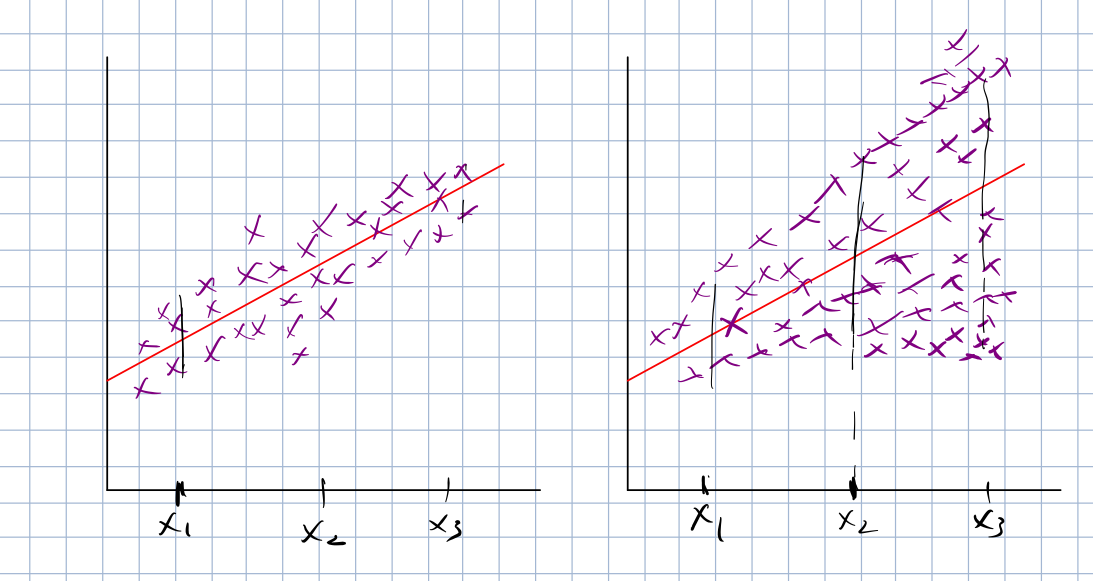
\includegraphics[width=0.55\textwidth]{hetero.png}
\end{figure}
\par\medskip
From the figure, we can see that the variance of the error term changes with $X_i$. In such case, standard errors of our estimators must take this into account. Running two versions of the regression in STATA would help. The homoskedastic version could be obtained by \texttt{regress y x}, while the heteroskedastic version requires \texttt{regress y x, vce(robust)} or \texttt{regress y x, robust}.  Below, I regressed the codes from the previous recitation for comparison. \par\medskip
\begin{figure}
\centering
\begin{subfigure}[H]{0.475\textwidth}
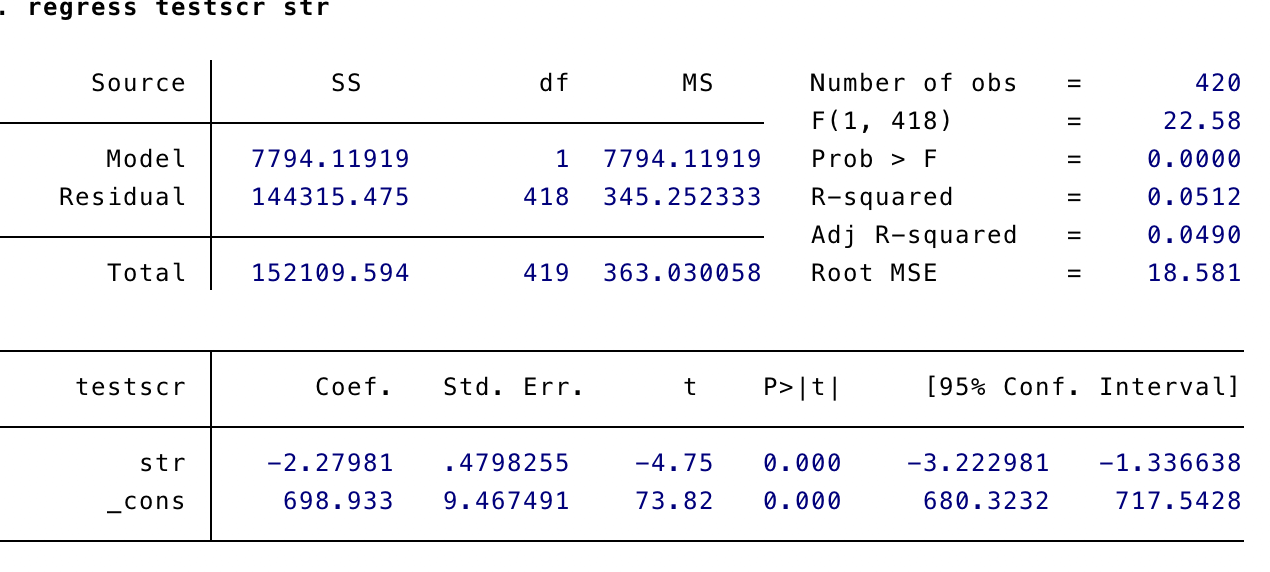
\includegraphics[width=\textwidth]{nonrobust.png}
\end{subfigure}
\begin{subfigure}[H]{0.475\textwidth}
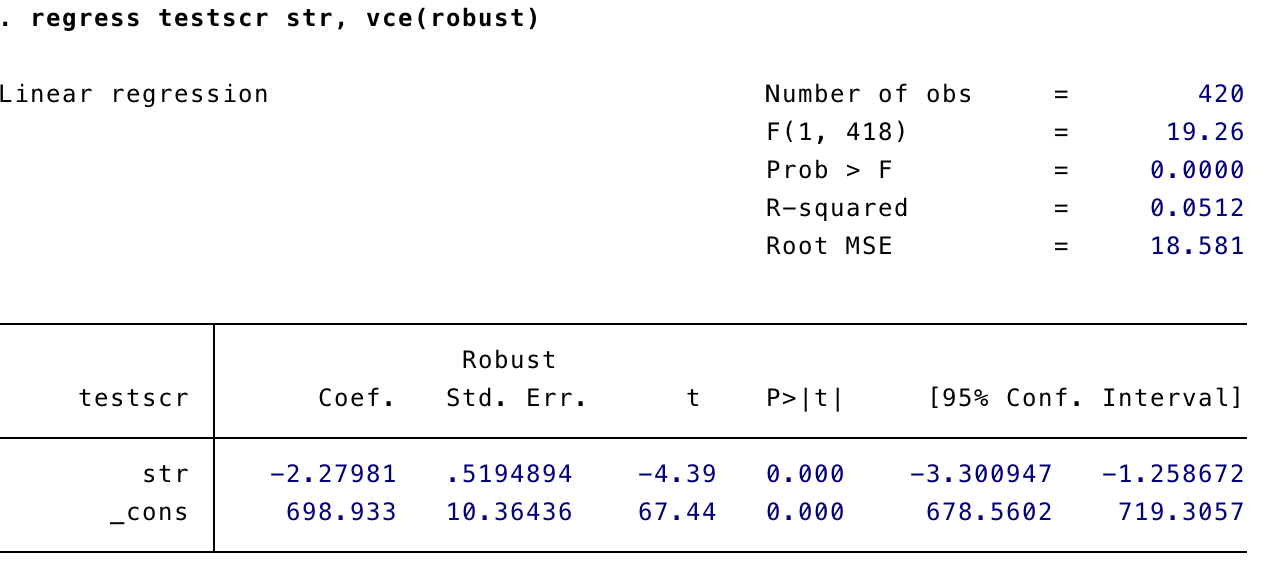
\includegraphics[width=\textwidth]{robust.png}
\end{subfigure}
\end{figure}
There are two takeaways from the picture
\begin{itemize}
\item \textbf{The variance rises (usually) in the heteroskedastic regression.} In other words, when we keep homoskedasticity assumption in cases where we should not do so, we end up rejecting null hypothesis that should not be rejected.
\item \textbf{The coefficients are unchanged.} When calculating the values for the estimators, we did not rely on the homoskedasticity assumption. Therefore, the coefficients are unaffected. In other words, the estimates are still unbiased.
\end{itemize}

\section{Multivariate regression models}
So far, we have assume that the number of our independent variable (other than the intercept term) is just one. We now extend our discussion to include more than one independent variable. 
\subsection{Omitted variable bias}
Before, we regressed whether test score is affected by the size of the classrooms. For every other factor that could affect the test score, we did not include them. However, one might guess that the higher the average income of a county, the higher the test score. Assume that this does affect the test score. Moreover, it is quite likely that richer neighborhoods can afford better school infrastructure and educational quality, leading to smaller size of classrooms. If this is the case, then the model that we have at the moment - without average income of the county - is not capturing the effect of classroom size on test score accurately. \par\medskip 
This is a case of an \textbf{omitted variable bias}. If there is an omitted variable bias, then the estimate we have of the effect of $X_i$ on $Y_i$ is not accurate and thus biased. One formal way to express this issue is as follows: Suppose that the true population regression model and the sample regression model is 
\[
\begin{aligned}
\text{True: }& Y_i = \beta_0 + \beta_1 X_i + \beta_2 Z_i+u_i\\
\text{Mistake: }& Y_i = \beta_0 + \beta_1 X_i + u_i^*\\
\text{Sample: }& Y_i = \hat{\beta}_0 + \hat{\beta}_1 X_i+ \hat{u}_i\\
\end{aligned}
\]
Suppose you run an OLS regression without $Z_i$. As discussed in previous lectures, the OLS estimator for $\beta_1$ can be calculated as $\frac{\sum_{i=1}^n(X_i-\bar{X})(Y_i-\bar{Y})}{\sum_{i=1}^n(X_i-\bar{X})^2}$. However, if you include the $(Y_i-\bar{Y})$ from the true regression model, the OLS estimator now becomes
\[
\begin{aligned}
\frac{\sum_{i=1}^n(X_i-\bar{X})(Y_i-\bar{Y})}{\sum_{i=1}^n(X_i-\bar{X})^2} =& \frac{\sum_{i=1}^n(X_i-\bar{X})(\beta_1(X_i-\bar{X})+\beta_2(Z_i-\bar{Z})+(u_i-\bar{u}))}{\sum_{i=1}^n(X_i-\bar{X})^2}\\
=& \beta_1 + \beta_2\frac{\sum_{i=1}^n(X_i-\bar{X})(Z_i-\bar{Z})}{\sum_{i=1}^n(X_i-\bar{X})^2}+\frac{\sum_{i=1}^n(X_i-\bar{X})(u_i-\bar{u})}{\sum_{i=1}^n(X_i-\bar{X})^2}\\
\end{aligned}
\]
Notice the term $\beta_2\frac{\sum_{i=1}^n(X_i-\bar{X})(Z_i-\bar{Z})}{\sum_{i=1}^n(X_i-\bar{X})^2}$. If $\beta_2 \neq0$ and $\frac{\sum_{i=1}^n(X_i-\bar{X})(Z_i-\bar{Z})}{\sum_{i=1}^n(X_i-\bar{X})^2}\neq 0$, then the mean of $\hat{\beta}_1$ is not guaranteed to be $\beta_1$. This is the reason why omitted variable bias causes inaccurate estimate of $\hat{\beta}_1$. These happen when both of the following cases hold
\begin{itemize}
\item \underline{$Z$ should explain $Y$}: If the slope coefficient of $Z$ is nonzero, then the $Z$ variable is part of the error term if we forget to include them
\item \underline{$Z$ is correlated with $X$}: If $cov(X,Z)\neq0$ and the regression residual $\hat{u}$ is correlated with $Z$, the independent variable is now correlated with $\hat{u}$, which leads to violation of the assumption that independent variable and the residual are not correlated.
\end{itemize} \par\medskip
If both conditions hold, the estimated effect of $X_1$, which is $\hat{\beta}_1$ is not unbiased and is inconsistent. This leads to the result where $E[u^*_i|X_i]=0$ assumption does not hold. There is a formal way to show this with equations.
\par\medskip
With the above formula, we can even determine the direction of the omitted variable bias - whether an estimate is biased downward or upward. The direction of the bias is determined by the sign of the $\beta_2\frac{\sum_{i=1}^n(X_i-\bar{X})(Z_i-\bar{Z})}{\sum_{i=1}^n(X_i-\bar{X})^2}$ term. If this term is positive, then the estimated $\hat{\beta}_1$ becomes larger than the true $\beta_1$. Thus, the estimate is said to be \textbf{overestimated}. If otherwise, $\hat{\beta}_1$ becomes smaller than the true $\beta_1$, making $\hat{\beta}_1$ \textbf{underestimated}.
\par\medskip
In order to address this issue, we can simply include the $Z$ variable if we have the data for it. Another way is to conduct an ideal randomized controlled experiment that randomly assigns \textit{str} to all students. If none of the two are feasible, we should find another variable that can be a proxy to $Z$ - they have to be related to the $X$ variable and is uncorrelated with the errors - which is the Instrumental Variable method. \par\medskip

\subsection{Multivariate Regression}
\textbf{Multivariate Regression} is simply a regression that involves more than one independent variables. The technicalities involved do not change drastically compared to the univariate regression. However, one should interpret the coefficients cautiously. Suppose that the regression is
\[
Y_i = \beta_0 + \beta_1 X_i + \beta_2 Z_i+u_i
\]
and the variable of interest is $X_i$. To see the impact of $X_i$ and $Y_i$, one needs to take (partial) derivatives on $Y_i$ with respect to $X_i$. This leads to
\[
\beta_1 = \frac{\partial Y_i}{\partial X_i}
\]
In words, $\beta_1$ captures how much $Y_i$ changes with respect to $X_i$ \emph{holding other variables constant} (ceteris paribus). If you do not hold other variables ($Z_i$ in this case) fixed, the change will not exactly be $\beta_1$ (it could be more or less). The statement \emph{holding other variables constant} is crucial in interpreting the $\beta_1$ coefficient.
\par\medskip


\subsection{Multivariate Regression: Sampling Statistics}
The estimates for the $\hat{\beta}_j, \ j\in\{0,1,2\}$ can be obtained in a similar way in which we have obtained the OLS estimates for the single variable version. Namely, solve the following minimization problem and get first order conditions with respect to $\beta_0, \beta_1, \beta_2$
\[
\min_{\{\beta_0,\beta_1,\beta_2\}} \sum_{i=1}^n[Y_i-\beta_0 - \beta_1X_{1i}-\beta_2X_{2i}]^2
\]
After some more amount of algebra (than the single variable case), the result we get is the following
\begin{itemize}
\item[$\hat{\beta}_0=$] $\bar{Y}-\hat{\beta}_1\bar{X}_1-\hat{\beta}_2\bar{X}_2$
\item[$\hat{\beta}_1=$] $\frac{\sum_{i=1}^n (X_{1i}-\bar{X}_1)(Y_{i}-\bar{Y})\sum_{i=1}^n(X_{2i}-\bar{X}_2)^2-\sum_{i=1}^n (X_{2i}-\bar{X}_2)(Y_{i}-\bar{Y})\sum_{i=1}^n(X_{1i}-\bar{X}_1)(X_{2i}-\bar{X}_2)}{\sum_{i=1}^n (X_{1i}-\bar{X}_1)^2\sum_{i=1}^n (X_{2i}-\bar{X}_2)^2-[\sum_{i=1}^n (X_{1i}-\bar{X}_1)(X_{2i}-\bar{X}_2)]^2}$
\item[$\hat{\beta}_2=$] $\frac{\sum_{i=1}^n (X_{2i}-\bar{X}_2)(Y_{i}-\bar{Y})\sum_{i=1}^n(X_{1i}-\bar{X}_1)^2-\sum_{i=1}^n (X_{1i}-\bar{X}_1)(Y_{i}-\bar{Y})\sum_{i=1}^n(X_{1i}-\bar{X}_1)(X_{2i}-\bar{X}_2)}{\sum_{i=1}^n (X_{1i}-\bar{X}_1)^2\sum_{i=1}^n (X_{2i}-\bar{X}_2)^2-[\sum_{i=1}^n (X_{1i}-\bar{X}_1)(X_{2i}-\bar{X}_2)]^2}$
\end{itemize} \par\medskip
However, what matters at this point is how we should interpret these coefficients. Suppose that we raise the amount of $X_{1i}$ and leave others unchanged. Then $Y_i$ changes by $\hat{\beta}_1$. Therefore, $\hat{\beta}_1$ measures the change in $Y_i$ due to change in $X_{1i}$ \emph{while leaving other independent variables constant} (ceteris paribus). If other variables are allowed to change, then the change in $Y_i$ due to change in $X_i$ by 1 unit is not guaranteed to be equal to $\hat{\beta}_1$.

\subsection{Multicollinearity}
When including more independent variables, we are quite likely to end up including independent variables that are highly correlated with each other. \textbf{Multicollinearity} refers to this situation. There are two types of multicollinearities. We say two variables $X_1$ and $X_2$ are \textbf{perfectly multicollinear} if $X_1$ is in an exact linear relationship of some sort with $X_2$. Any multicollinearities that are not in exact linear relationship is referred to as \textbf{imperfect multicollinearity}. \par\medskip

When there is a perfect multicollinearity, we run in to the situation where the denominator and the numerator of the OLS estimates is not defined. These two cases demonstrate possible consequences of multicollinearity
\begin{itemize}
\item \textbf{Assume that $X_2 = cX_1$ for some constant $c$}: Then we have $(X_{2i}-\bar{X}_2)=c(X_{1i}-\bar{X}_1)$. Then $\hat{\beta}_1$ changes to
\scriptsize{\begin{gather*}
\frac{\sum_{i=1}^n (X_{1i}-\bar{X}_1)(Y_{i}-\bar{Y})c^2\sum_{i=1}^n(X_{1i}-\bar{X}_1)^2-c\sum_{i=1}^n (X_{1i}-\bar{X}_1)(Y_{i}-\bar{Y})c\sum_{i=1}^n(X_{1i}-\bar{X}_1)(X_{1i}-\bar{X}_1)}{\sum_{i=1}^n (X_{1i}-\bar{X}_1)^2 c^2\sum_{i=1}^n (X_{1i}-\bar{X}_1)^2-c^2[\sum_{i=1}^n (X_{1i}-\bar{X}_1)(X_{1i}-\bar{X}_1)]^2} \\
=\frac{0}{0} = ???
\end{gather*}}\normalsize
Therefore, $\hat{\beta}_1$ will not be defined (similar for $\hat{\beta}_2$).
\item \textbf{Dummy variable trap}: Say that you have the dummy variable for females and males. Let each of them be $X_{1i}$ and $X_{2i}$ with $X_{2i}=1-X_{1i}$. Then the regression can be written as
\begin{gather*}
Y_i = \beta_0 + \beta_1X_{1i} + \beta_2X_{2i} + u_i \iff Y_i = \beta_0 + \beta_1X_{1i} + \beta_2(1-X_{1i}) + u_i \\
\iff Y_i = \beta_0 + \beta_2 +(\beta_1-\beta_2)X_{1i}+u_i
\end{gather*}
Therefore, by including both $X_{1i}$ and $X_{2i}$ in the same regression, the $X_{2i}$ vanishes from the equation. This is why when you have dummy variables for all categories in the observation, one of them must be left out.
\end{itemize} \par\medskip
The STATA deals with perfect multicollinearity by dropping out some variables that cause perfect multicollinearity.

%%%%%%%%%%%%%%%%%%
\subsection{Joint testing: Types of Hypothesis Testing}
We have covered hypothesis tests since the beginning of this course. In the regression with single independent variable, we have used $t$-distribution (or if $n$ is sufficiently large, normal distribution) to check whether the following hypothesis hold:
\[
H_0 : \beta_1 = 0 \ \ H_1 : \beta_1 \neq 0
\]
and the test statistic was (assuming homoskedasticity)
\[
t=\frac{\hat{\beta}_1-0}{s.e(\hat{\beta})}\sim t_{n-2} \ \ (\sim N(0,1) \ \text{in large samples})
\]
where $s.e(\hat{\beta}_1)=\sqrt{\frac{1}{n}\frac{\frac{1}{n-2}\sum_{i=1}^n(X_i-\bar{X})\hat{u}_i}{(\frac{1}{n}\sum_{i=1}^n (X_i-\bar{X})^2)^2}}$. So it may seem plausible to think that to test the hypothesis on a setting where we have multiple independent variables, we just need to run this many times. However, this is not exactly the case. the following example demonstrates why. \\ \par

\begin{mdframed}[backgroundcolor=blue!5] 
\textbf{Why do multiple testing using $t$-statistics have problems?} \medskip \\ 
Consider the case where there is you are testing on multiple independent variables. Suppose that you are running a two-sided test with 5 independent variables and significance level $\alpha = 5\%$ under the null hypothesis
\[
H_0: \beta_1=...\beta_5=0
\]
You reject the null hypothesis when $|t_i|\geq 1.96 \ i\in\{1,2,3,4,5\}$ Note that for each $i$, the probability of $|t_i|\geq 1.96$ is 0.05. Now assume that each test statics are independent. Then the probability of incorrectly rejecting the null hypothesis using this approach is
\[
\begin{aligned}
\Pr(|t_1|>1.96 \cup...\cup |t_5|>1.96) & =1-\Pr(|t_1|\leq1.96\cap .. \cap|t_1|\leq1.96)\\
(\because\text{Independence of $t_i$'s}) \ \ &=1-\Pr(|t_1|\leq1.96)\times ..\times\Pr(|t_5|\leq1.96) \\
 & = 1-(0.95)^5 \\
 &= 0.2262
\end{aligned}
\]
This means that the rejection rate under the null is not 5\% but 22\% percent. Therefore, we end up rejecting the null hypothesis more than we have to. (Formally, we say that the probability of type 1 error rises sharply.) 
\end{mdframed} \par\medskip
Because of this fact, we require another approach when testing multiple hypotheses at the same time. This is where \textbf{$F$-test} comes in. This is a test where all parts of the joint hypothesis can be tested at once. It also has mechanism for correcting the correlation between the $t$-test statistics. It ultimately allows us to correctly set the significance level even for the multiple testing case. \par\medskip
The usual joint hypothesis test for the regression with $k$ variables (not including the constant term) is
\[
H_0: \beta_1 = ... =\beta_k=0, \ H_1:\lnot H_0
\]
where $H_1$ refers to the case where there is a nonzero element in any one of $\beta_1$ to $\beta_k$. The $\lnot$ symbol refers to ``not". Note that the default F-test null hypothesis for STATA is $H_0:\beta_1 = ... =\beta_k=0$ and $H_1: \lnot H_0$.\par\medskip
We can actually go farther. Suppose that instead of $\beta_1$ and $\beta_2$ being zero, we are just interested in whether they are equal. The $F$-test can also be used for testing this hypothesis. The setup of the hypothesis would be
\[
H_0: \beta_1 = \beta_2 \ H_1: \beta_1 \neq \beta_2
\]
I will discuss how to implement such hypothesis test on STATA in the next section. \par\medskip
\noindent
\textit{For curious minds: } Note that the square of the $t$ distribution with the degree of freedom $n$ is equivalent to the $F$ distribution with $1$ degree of freedom in the numerator and $n$ in the denominator. For more information, please refer the link I attach in the footnotes\footnote{\url{http://homepage.stat.uiowa.edu/~rdecook/stat3200/notes/t_and_F_4pp.pdf}}
\subsection{Interpreting the Results}
Below are the results of a regression on multiple variables. I am using the data from Professor Almond's paper on cost of low birthweight\footnote{Almond, Douglas, Kenneth Chay, David Lee (2005) ``The Costs of Low Birthweight", \textit{Quarterly Journal of Economics} 120(3):1031-1083}. I regress \textit{birthweight} on \textit{smoker, alcohol, Nprevist} (number of prenatal visits to doctor).
\begin{figure}[H]
\begin{center}
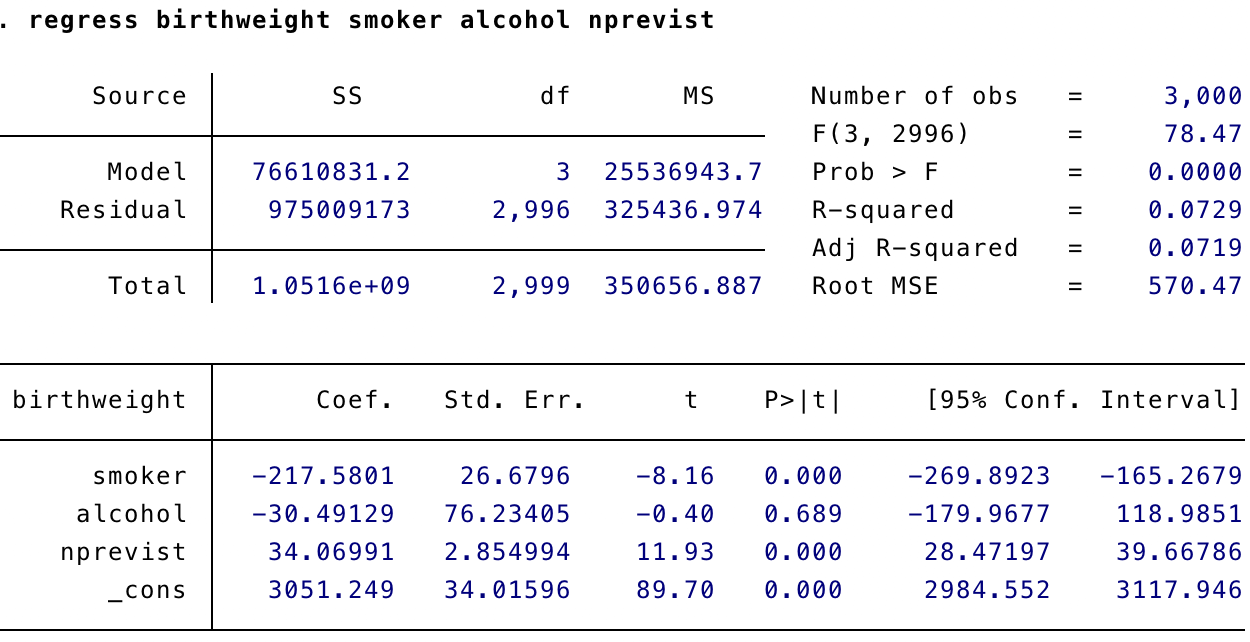
\includegraphics[width=0.7\textwidth]{regoutput.png}
\end{center}
\end{figure}\par\medskip
You can see that running multivariate regression is similar in terms of the techniques involved. Additional complication rises from interpreting the goodness of fit. In addition to $R^2$, we now get the \textbf{adjusted $R^2$}, which is defined as
\[
\bar{R}^2 = 1-\frac{n-1}{n-k-1}\frac{\text{Residual Sum of Squares}}{\text{Total Sum of Squares}}
\]
Since we are assuming that $k\geq 1$, adjusted $R^2$ is smaller than the $R^2$. As we include more variables, the $\frac{n-1}{n-k-1}$ increases, leading to further decrease in adjusted $R^2$. However, if the new variables are very relevent, $\frac{\text{Residual Sum of Squares}}{\text{Total Sum of Squares}}$ decreases. This reduces the gap between $R^2$ and the adjusted $R^2$. If the adjusted $R^2$ do not decrease drastically, it is a sign that we are adding a relevant variable. \par\medskip
One way to conduct various hypothesis testing is to utilize the \texttt{test} command. I include two pictures, one with $H_0: \beta_{\text{smoker}}=\beta_{\text{alcohol}}=\beta_{\text{nprevist}}=0$ on the left and the other with $H_0:\beta_{alcohol}+\beta_{nprevist}=0$ on the right.
\begin{figure}[H]
\begin{center}
        \begin{subfigure}[b]{0.45\textwidth}
	\centering
                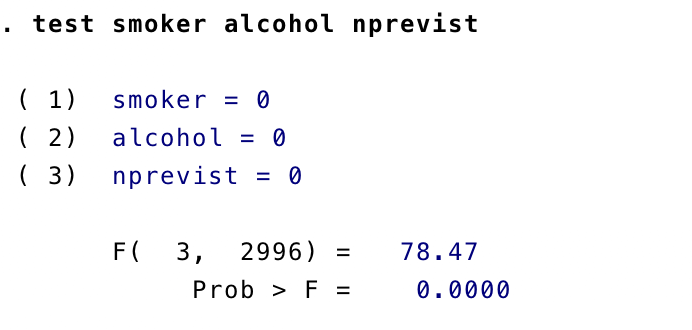
\includegraphics[width=\linewidth]{test}
        \end{subfigure}
        \begin{subfigure}[b]{0.45\textwidth}
	\centering
                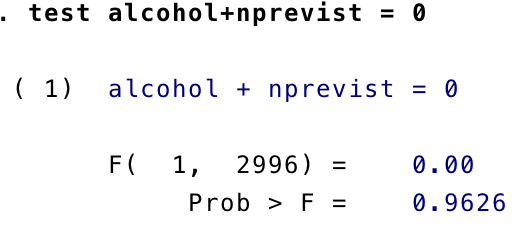
\includegraphics[width=\linewidth]{test1}
        \end{subfigure}
\end{center}
\end{figure}



%%%%%%%%%%%%%%%%%%
\subsection{F-tests}
You should know after the problem sets that you use $F$-tests to assess the results of a joint hypothesis. The \textbf{$F$-statistics} are calculated in two ways. One uses $t$-statistics from individual hypotheses. This is calculated as
\[
\frac{1}{2}\left(\frac{t_1^2+t_2^2-2\hat{\rho}_{t_1,t_2}t_1t_2}{1-\hat{\rho}^2_{t_1,t_2}}\right)
\]\par\medskip
Another one, which is useful for calculating $H_0: \beta_1 = ... =\beta_q=0$ hypothesis ($q$ is the number of hypotheses being tested on) uses $R^2$ from the 'unrestricted' and 'restricted' regressions. Assume that there are total of $k$ independent variables, where $k\geq q$ and the null hypothesis is as stated above. The restricted regressions and unrestricted regressions are defined as
\[\begin{aligned}
\text{Restricted: } & Y_i =\beta_0+ 0X_{1,i} + ...+ 0X_{q,i}+ \beta_{q+1}X_{q+1,i}+...+\beta_kX_{k,i} + u_i\\
\text{Unrestricted: } & Y_i = \beta_0+\beta_1X_{1,i} + ... +\beta_qX_{q,i}+ \beta_{q+1}X_{q+1,i}+...+\beta_kX_{k,i} + u_i\\
\end{aligned}\] \par\medskip
You can now notice that restricted regression assumes that $H_0$ is true and then only optimizes with respect to $\beta_{q+1},...,\beta_{k}$. Unrestricted regression does not assume that $H_0$ is true and optimizes with respect to all slope coefficients. The second formula for $F$-statistic uses $R^2$ from these two regressions. Intuitively, the unrestricted regression allows for the role of $X_1,..,X_q$ whereas their role in restricted regression is limited. This is why $R^2$ in unrestricted regression is higher than restricted regression. Given this, $F$-statistic is
\[
\frac{(R^2_{\text{Unrestricted}}-R^2_{\text{Restricted}})/q}{(1-R^2_{\text{Unrestricted}})/(n-k-1)}
\]
where $k$ is total number of independent variables (not counting intercept) and $q$ is the number of restrictions. \par\medskip
There is another way to express this. Note that $R^2_{\text{Restricted}} = 1-\frac{RSS_{\text{Restricted}}}{TSS}$. $R^2_{\text{Unrestricted}}$ is defined similarly. By using this and with little algebra, we can derive this formula, which is mentioned in most econometrics textbooks.
\[
\frac{(RSS_{\text{Restricted}}-RSS_{\text{Unrestricted}})/q}{(RSS_{\text{Unrestricted}})/(n-k-1)}
\] \par\medskip


\subsection{Control variables and conditional mean independence}
Assume that we have a following setup:
\[
\begin{aligned}
\text{True: }& Y_i = \beta_0 + \beta_1 X_i + \beta_2 Z_i+u_i\\
\text{Mistake: }& Y_i = \beta_0 + \beta_1 X_i + u_i^*\\
\text{Sample: }& Y_i = \hat{\beta}_0 + \hat{\beta}_1 X_i+ \hat{u}_i\\
\end{aligned}
\]
If we end up with an omitted variable bias by not including $Z_i$, Then, we have a problem. We can see this from
\[
\begin{aligned}
E[u_i^*|X_i]&=E[\beta_2Z_i+u_i|X_i]\\
&=\beta_2Z_i+E[u_i|X_i] \neq 0
\end{aligned}
\]
So Assumption 2 from the classical linear regression model (refer to Recitation 3), fails and $\hat{\beta}_1$ without inclusion of $Z_i$ is biased. To address this, we ideally add this variable into the regression. That may not always be possible. In that case, we can find $W_i$ variable that is correlated with $Z_i$ to some extent and include that in the regression. By doing so, we achieve three things
\begin{itemize}
\item The $u_i$ term is no longer correlated with $X_i$ ($cov(X_i, u_i)=0$)
\item For given value of $W_i$, then the variable of interest $X_i$ is no longer correlated with the omitted determinant of $Y_i$
\item For given $W_i$, $X_i$ acts as if they are randomly assigned
\end{itemize}
Variable $W_i$ that achieves this is called an \textbf{effective control variable}. In this particular case, we say that the \textbf{conditional mean independence} hold, in the sense that as long as we control for $W_i$, $u_i$ is independent of $X_i$ - making our coefficient of interest unbiased. 
\[
E[u_i|X_i,W_i]= E[u_i|W_i]
\]
Note that $W_i$ itself does not need to have causal relationship with $Y_i$


%%%%%%%%%%%%%%%%
\end{document}

